\documentclass[a4paper,openany,oneside,12pt]{book}
\usepackage[UKenglish]{babel}
\usepackage[UKenglish]{isodate}
\usepackage{graphicx}
\usepackage[utf8]{inputenc} % Para poner acentos y eñes directamente.
\usepackage{pdfpages}
\usepackage{listings}
\usepackage[T1]{fontenc}
\usepackage{hyperref}
\usepackage{algorithm2e}
\usepackage{url}
\usepackage{tikz}
\usetikzlibrary{arrows,positioning}

% Defines a `datastore' shape for use in DFDs.  This inherits from a
% rectangle and only draws two horizontal lines.
\makeatletter
\pgfdeclareshape{datastore}{
  \inheritsavedanchors[from=rectangle]
  \inheritanchorborder[from=rectangle]
  \inheritanchor[from=rectangle]{center}
  \inheritanchor[from=rectangle]{base}
  \inheritanchor[from=rectangle]{north}
  \inheritanchor[from=rectangle]{north east}
  \inheritanchor[from=rectangle]{east}
  \inheritanchor[from=rectangle]{south east}
  \inheritanchor[from=rectangle]{south}
  \inheritanchor[from=rectangle]{south west}
  \inheritanchor[from=rectangle]{west}
  \inheritanchor[from=rectangle]{north west}
  \backgroundpath{
    %  store lower right in xa/ya and upper right in xb/yb
    \southwest \pgf@xa=\pgf@x \pgf@ya=\pgf@y
    \northeast \pgf@xb=\pgf@x \pgf@yb=\pgf@y
    \pgfpathmoveto{\pgfpoint{\pgf@xa}{\pgf@ya}}
    \pgfpathlineto{\pgfpoint{\pgf@xb}{\pgf@ya}}
    \pgfpathmoveto{\pgfpoint{\pgf@xa}{\pgf@yb}}
    \pgfpathlineto{\pgfpoint{\pgf@xb}{\pgf@yb}}
 }
}
\makeatother



\newcommand{\textsharp}{$\sharp$}

\begin{document}

%titlepage
\thispagestyle{empty}
\begin{center}
\begin{minipage}{0.75\linewidth}
    \centering
%University logo
    
\includegraphics[height=1.5cm]{img/logo-upv}\\
    \vspace{2cm}
%Thesis title
    {\uppercase{\Large Audio Classical Composer Identification in MIREX 2015: Submission based on Structural Analysis of Music\par}}
    \vspace{2.5cm}
%Author's name
    {\Large Leopoldo Pla Sempere\par}
        {\it leoplsem@posgrado.upv.es}\\
        Polytechnic University of Valencia\\
        \vspace{1cm}
        {\uppercase {Departament of Computer Systems and Computation}}\\
        \vspace{0.5cm}
        {\it Supervised by: Roberto Paredes Palacios}\\
        \vspace{0.5cm}
        Master's Degree in Artificial Intelligence, Pattern Recognition and Digital Imaging\\
    \vspace{2cm}
%Degree
    {\Large M.Sc. Thesis\par}
    \vspace{2cm}
%Date
\date{\today}
    {\today}
\end{minipage}
\end{center}
\clearpage



\newpage
\mbox{}
\thispagestyle{empty} % para que no se numere esta pagina



\chapter*{License}
Documents are licensed under Creative Commons Attribution - ShareAlike 4.0 International (CC BY-SA).

\url{http://creativecommons.org/licenses/by-sa/4.0/}



Source code under GNU GENERAL PUBLIC LICENSE (GPL).

\url{http://www.gnu.org/copyleft/gpl.html}


\begin{figure}
\centering

\includegraphics{img/cc.png} 

This work is licensed under a Creative Commons Attribution-ShareAlike 4.0 International License.
\end{figure}


\newpage
\thispagestyle{empty}
\mbox{}


\chapter*{}
\begin{flushright}
\textit{Dedicado a \\
Laura}
\end{flushright}


\newpage
\thispagestyle{empty}
\mbox{}


\chapter*{Abstract}
\addcontentsline{toc}{section}{Abstract} % si queremos que aparezca en el índice
\markboth{ABSTRACT}{ABSTRACT} % encabezado

This work is the result of interest in neural networks and classical music, knowledge that I wanted to combine after finishing the studies of the IARFID master and professional music degree. I wanted to contribute to an engineering task from the musicological point of view, so, after working on PAN 2015 author profiling task and learning about sentiment analysis, I concluded that I could use similar techniques in MIREX classical composer identification task.

MIREX is the Music Information Retrieval Evaluation eXchange organized by the University of Illinois at Urbana-Champaign (UIUC) in which every year they prepare several Music Information Retrieval tasks held as part of the International Conference on Music Information Retrieval (ISMIR), which this year is celebrated in Malaga. In this exchange exist the Audio Classification (Train/Test) Tasks, and more specifically the Audio Classical Composer Identification, which is perfect for investigating the use of machine learning and music analysis on classical music.

Machine learning is a field of the artificial intelligence which evolves from the study of pattern recognition and include the study of algorithms that can learn and make decisions over data. Specifically, a neural network is a machine learning algorithm that is inspired by the biological neural networks.

Musical analysis is the process whereby a music piece is decomposed and understood as we analyze a text. There is no exact method for these analysis and differs from analyst to analyst. The lowest level of this musical analysis is the harmonic and functional analysis and a higher one is the structure of the segmentation.

This investigation includes the development of the idea and the software that implements the preprocessing and the classification of samples using different software technology layers, as Sonic Annotator, MATLAB and Bash scripts.


\newpage
\thispagestyle{empty}
\mbox{}



\tableofcontents % indice de contenidos

\cleardoublepage
\addcontentsline{toc}{chapter}{List of Figures} % para que aparezca en el indice de contenidos
\listoffigures % indice de figuras


\newpage
\thispagestyle{empty}
\mbox{}
\setlength{\parskip}{\baselineskip}



\chapter{Introduction} % Puede que la tenga que reescribir para no publicar esta idea de forma explícita
\pagenumbering{arabic} % para empezar la numeración con números
In the last years, Music Information Retrieval fields have been improving step by step and the majority of these fields are still using low level features of the audio signal. In computational linguistics authorship attribution, is usual to use features from the text representation as character measures, lexical measures and syntactic features. In fact, one of the features that the winner of PAN 2014 in the authorship task\cite{pan14} and most of author profiling task submissions in 2013\cite{pan13} use is the POS tagging of the text.

So, in this project I approximate the idea of musical structure analysis of classical audio files to identificate composers. This whole concept could be compared to apply POS tagging and segmentation to a speech recording.

Then, here we will focus on techniques of musical analysis, composition and machine learning instead of signal processing because none of the previous works in the author identification submissions of MIREX used this kind of high level features.

\section{MIREX}
The Music Information Retrieval Evaluation eXchange (MIREX) edition of 2015 is organized by The International Music Information Retrieval Systems Evaluation Laboratory (IMIRSEL) at the Graduate School of Library and Information Science (GSLIS), University of Illinois at Urbana-Champaign (UIUC). It's hold as part of the 16th International Conference on Music Information Retrieval, ISMIR 2015, which will be held in Malaga, Spain, October 26th-30th, 2015.

This exchange has several kind of tasks related to Music Information Retrieval:

\begin{itemize}
    \item Grand Challenge on User Experience
    \item Audio Classification (Train/Test) Tasks, incorporating:
    \begin{itemize}
        \item Audio US Pop Genre Classification
        \item Audio Latin Genre Classification
        \item Audio Music Mood Classification
        \item Audio Classical Composer Identification
        \item Audio K-POP Mood Classification
        \item Audio K-POP Genre Classification 
    \end{itemize}
    \item Audio Cover Song Identification
    \item Audio Tag Classification
    \item Audio Music Similarity and Retrieval
    \item Symbolic Melodic Similarity
    \item Audio Onset Detection
    \item Audio Key Detection
    \item Real-time Audio to Score Alignment (a.k.a Score Following)
    \item Query by Singing/Humming
    \item Audio Melody Extraction
    \item Multiple Fundamental Frequency Estimation \& Tracking
    \item Audio Chord Estimation
    \item Query by Tapping
    \item Audio Beat Tracking
    \item Structural Segmentation
    \item Audio Tempo Estimation
    \item Discovery of Repeated Themes \& Sections
    \item Audio Downbeat Estimation
    \item Audio Fingerprinting
    \item Singing Voice Separation 
\end{itemize}

This work is oriented to the Audio Classification (Train/Test) Task of Audio Classical Composer Identification.

\section{State of the Art}
Since this work is focused on MIREX exchange, the state of the art is easily obtainable because all the papers and submissions from previous years are stored and classified in the MIREX Wiki\cite{mirexWiki} and also lots of materials of the ISMIR proceedings\cite{ismirProc}.

For the specific task of Classical Composer Identification in MIREX 2014 the machine learning algorithms used were Convolutional Neural Networks (CNN)\cite{qiuqiang} and multiclass Support Vector Machines (SVM)\cite{seung-ryoel}\cite{shumin}\cite{ming}\cite{byun}, also using PCA\cite{shumin} and a SVM ranker\cite{seung-ryoel} as a dimensional reduction algorithm. Previous years there were used Restricted Boltzmann Machines (RBM)\cite{pikrakis}, Gaussian Mixture Models (GMM)\cite{franz}, k-Nearest Neighbours classifier (kNN) and Multi Layer Perceptron (MLP)\cite{hamel}. In general, SVM is the most used technique for this task.

From the features point of view, the most used features are timbral features as mel-frequency cepstral coefficients (MFCC)\cite{seung-ryoel}\cite{byun}\cite{franz}, decorrelated filter banks (DFB)\cite{seung-ryoel}\cite{byun} and octave-based spectral contrast (OSC)\cite{seung-ryoel}\cite{byun}, visual features as spectograms\cite{seung-ryoel}, spectral patterns (SP)\cite{klaus}, Delta spectral patterns (DSP)\cite{klaus} and Short Time Fourier Transform (STFT)\cite{qiuqiang}\cite{shumin}, and also rhythmic patterns as Logarithmic Fluctuation Patterns (LFP)\cite{klaus} and Correlation Patterns (CP)\cite{klaus}. After the extraction of these features, sometimes are preprocessed before using them in the machine learning system with some statistical features as mean and variance of the timbral features\cite{seung-ryoel} or with Gabor filters\cite{ming12}, as it is usually done in Biometrics and Computer Vision.

\begin{figure}
\centering
   \begin{tabular}{ | l || l | }
   \hline
   Algorithm & Normalised Classification Accuracy \\ \hline
   BK1 & 0.6876 \\ \hline
   SS6 & 0.6732 \\ \hline
   SSKS1 & 0.6728 \\ \hline
   WJ2 & 0.6089 \\ \hline
   QK2 & 0.5685 \\ \hline
   BK2 & 0.5213 \\ \hline
   BK3 & 0.4015 \\ \hline
   BK4 & 0.3947 \\ \hline
   XG3 & 0.3312 \\ \hline
   XG2 & 0.3312 \\ \hline
   \end{tabular}

\caption{Normalised Classification Accuracies of MIREX 2014.\cite{resultsMirex14}} \label{fig:MIREX14results}
\end{figure}

Note that most of the submissions for Composer Classification task were also submitted for all Audio Classification (Train/Test) Tasks, so they are relatively generic audio classifiers algorithms.

\section{Neural Networks}

One of the most famous techniques of machine learning nowadays is the neural network topology.

An artificial neural network is a class of classification program that is trained to solve problems by learning the features of the problem through a set of already classified data, or labeled training set. This specific kind of software is designed based on the study of how biologic brain works and it has lots of applications in computer vision, speech recognition, natural language processing, bioinformatics and many other science sectors.



\begin{quote}
\em The word network in the term 'artificial neural network' refers to the inter-connections between the neurons in the different layers of each system. An example system has three layers. The first layer has input neurons which send data via synapses to the second layer of neurons, and then via more synapses to the third layer of output neurons. More complex systems will have more layers of neurons, some having increased layers of input neurons and output neurons. The synapses store parameters called "weights" that manipulate the data in the calculations.

An ANN is typically defined by three types of parameters:
\begin{itemize}
\item The interconnection pattern between the different layers of neurons
\item The learning process for updating the weights of the interconnections
\item The activation function that converts a neuron's weighted input to its output activation.
\cite{wiki:ann}
\end{itemize}
\end{quote}


\begin{figure}
\centering
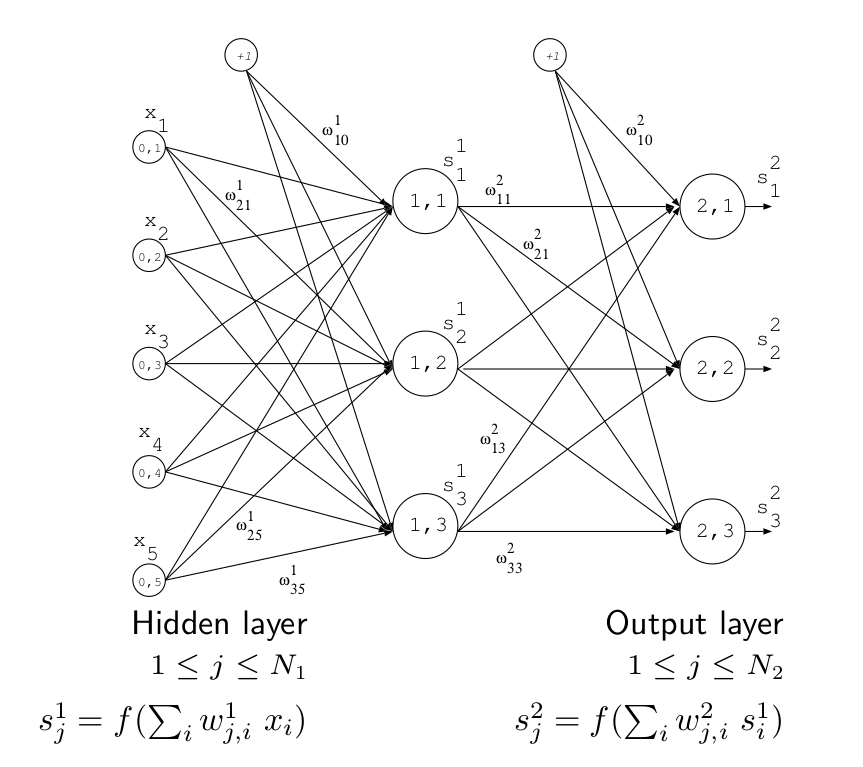
\includegraphics[width=0.8\textwidth]{img/neuralNet.png} 
\caption{General structure of a multilayer perceptron\cite{rparedesNN}} \label{fig:neuralnet}
\end{figure}

Also, this kind of topology is easily paralelizable and it has been implemented in so many frameworks that use several CPU and GPU cores (CUDA or OpenCL, for example).

The origin of the artificial neural networks can be stablished at the first models defined with mathematical notation by McCullock and Pitt in 1943, but the first successful results are obtained in 1959 when the perceptron is created by Rosenblat, which later in 1975 is improved by Paul Werbos adding the backpropagation algorithm.

In the last years, the use of this type of learning algorithms has increased compared to the Radial Basis Functions or the Support Vector Machines algorithms, caused by the "boom" of the Deep Learning and the Convolutional Networks.

Nowadays, the most used artificial neural networks are the Restricted Boltzmann Machines, the Convolutional Neural Networks and the Deep Belief Networks.

\subsection{Unsupervised Learning}
As Bishop states in his book "Pattern Recognition and Machine Learning":
\begin{quote}
\em In other pattern recognition problems, the training data consists of a set of input vectors x without any corresponding target values. The goal in such unsupervised learning problems may be to discover groups of similar examples within the data, where it is called clustering, or to determine the distribution of data within the input space, known as density estimation, or to project the data from a high-dimensional space down to two or three dimensions for the purpose of visualization.\cite{Bishop}
\end{quote}

In short, unsupervised learning is a learning technique focused on finding hidden structure in unlabeled data as k-Nearest-Neighbours or Autoencodes do. This last one is used by Deep Belief Networks to pretrain an Artificial Neural Network. 

\subsection{Deep Belief Network}

The Deep Belief Network is a subtype of Artificial Neural Networks inside the Deep Learning algorithms, which is based on a set of hidden units layers with unsupervised learning. These layers try to reconstruct the data layer by layer and a final set of layers, that are treated as a Multi Layer Perceptron, are trained with labeled data using backpropagation.
\begin{quote}
\em The top two layers have undirected, symmetric connections between them and form an associative memory. The lower layers receive top-down, directed connections from the layer above. The states of the units in the lowest layer represent a data vector.

The two most significant properties of deep belief nets are:

\begin{itemize}
\item There is an efficient, layer-by-layer procedure for learning the top-down, generative weights that determine how the variables in one layer depend on the variables in the layer above. 

\item After learning, the values of the latent variables in every layer can be inferred by a single, bottom-up pass that starts with an observed data vector in the bottom layer and uses the generative weights in the reverse direction.\cite{Hinton:2009}
\end{itemize}
\end{quote}

Since the final result is a MLP, the main difference of DBN with a simple MLP is that this MLP is initialized with the reconstructed data of the DBN which usually obtains better results.


\begin{figure}
\centering
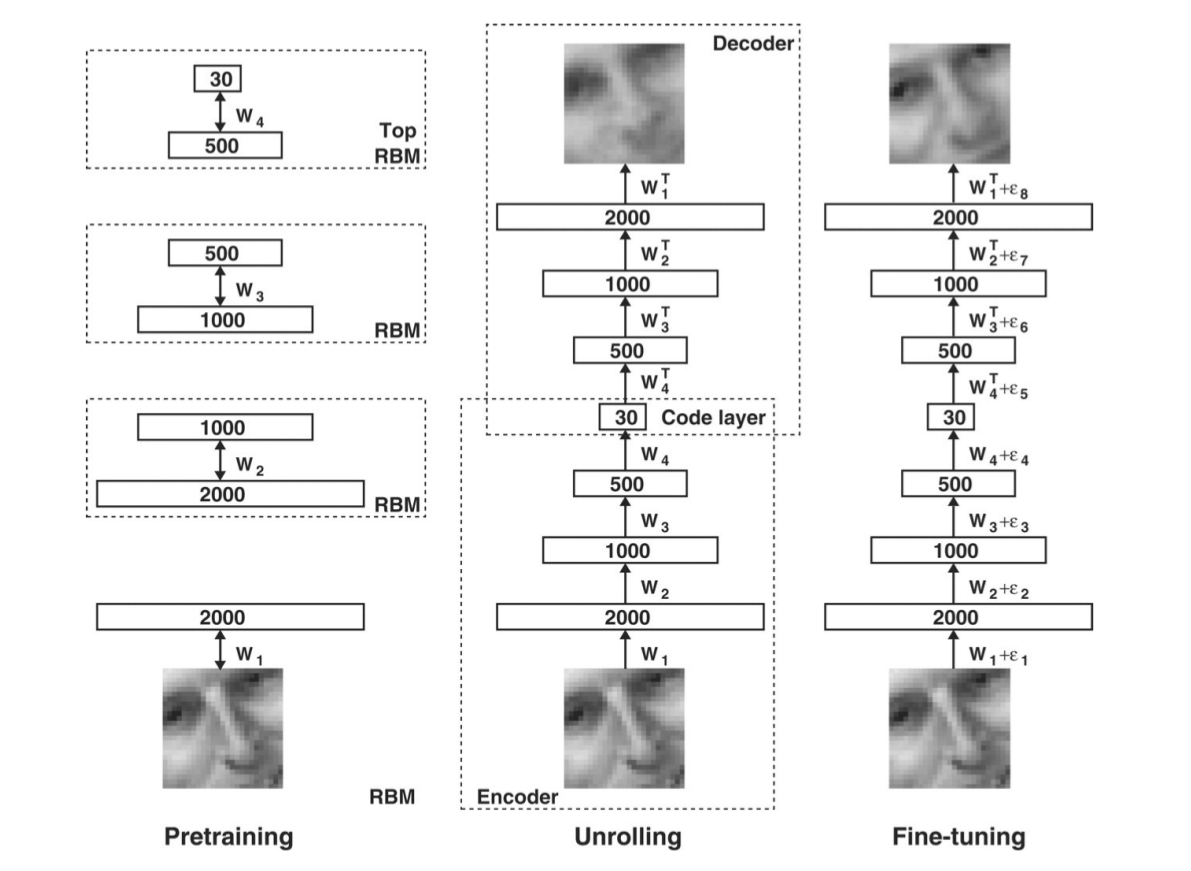
\includegraphics[width=0.7\textwidth]{img/dbn_model.png} 
\caption{Deep Belief Network training example\cite{rparedesNN}} \label{fig:dbn}
\end{figure}


\subsection{Musical analysis}
The process and the academic discipline which studies the musical works from the pattern aspect, the internal structure, composition techniques and interpretative aspects is the musical analysis.

The basic objectives of the musical analysis are the recognition of different elements of the work

\begin{itemize}
\item Structure
\item Melody
\item Texture
\item Harmony
\item Tone
\item Dynamic
\end{itemize}

Also, to study the relationships inside the previous elements and between them. And finally obtain conclusions about the relationships, the compositor ideas and why the composer structured the elements in that way.

Usually, the musical analysis is performed over a score because is easier to identify the elements, but also listening to parts of the work is sometimes needed.

This analysis include different subanalysis or techniques that are used to describe the musical work:

\begin{itemize}
\item Discretization: breaking the piece down into smaller parts and examine the way these parts are connected. In fact, Fred Lerdahl\cite{Lerdahl} argues that discretization is indispensable for a musical analysis.
\item Harmonic analysis: indicate the harmonic functions on the same score including figured bass and modulations if harmony is tonal.
\end{itemize}

When the discretization is more intuitive to perform, the harmonic analysis implies the knowledge of the harmonies in different scales\ref{fig:scalesharmonies}. Also, the knowledge of the most famous cadences is very important. These are some:

\begin{itemize}
\item Perfect Authentic Cadence (PAC): V to I (chords in root position)
\item Imperfect Authentic Cadence (IAC): V to I (with modified notes)
\item Half Cadence (HC): V of V, ii, vi, IV, or I to V
\item Plagal Cadence (PC): IV to I
\item Interrupted Cadence: V to vi
\end{itemize}

Also there are more cadences and larger common progressions, like "I IV I IV" or "I IV V7 I" that are interesting to note\cite{jacmuse}.

\begin{figure}
\centering
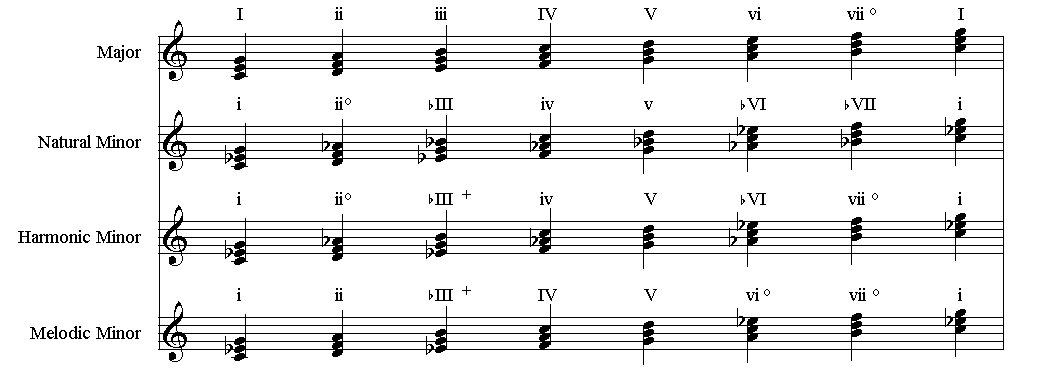
\includegraphics[width=\textwidth]{img/scales.png} 
\caption{Figured bass in different scales of C} \label{fig:scales}
\end{figure}

As an illustrative example, looking at this Beethoven Minuet\ref{fig:music_analysis} we can see the letters above the staff that denotes the different sections of the score. We obtained "a", "b", "c" and again "b". Also, we made the harmonic analysis ("I", "V", "IV" and the other variants and elements below the staff) focusing on cadences like Half Cadence (HC), Perfect Authentic Cadence (PAC) or Imperfect Authentic Cadence (IAC). There are more elements like passing tones (PT) and subjective descriptions.

This field of the music theory covers music from medieval era to the contemporary music, but in this work we are focused on classical music analysis and the application of the techniques that we showed in the example.

\begin{figure}
\centering
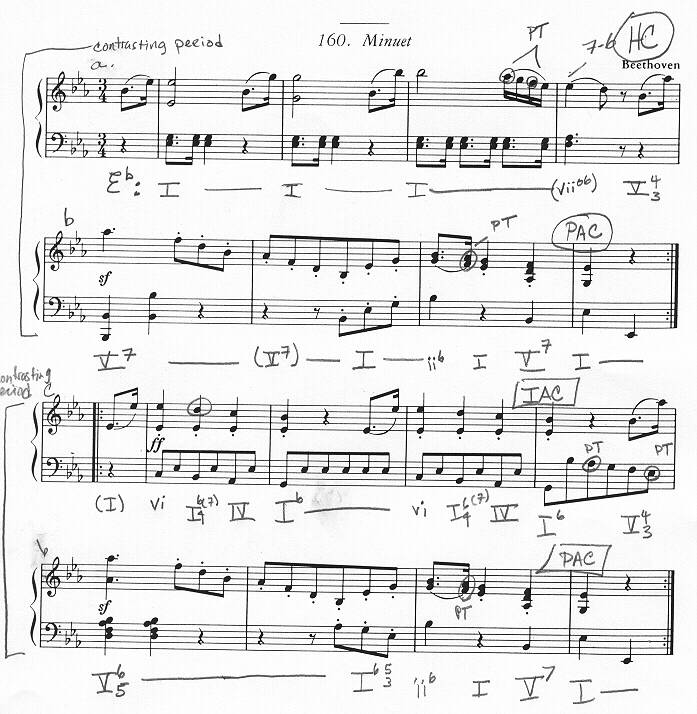
\includegraphics[width=0.9\textwidth]{img/musical_analysis.jpg} 
\caption{Analysis of a Beethoven Minuet No. 3. of 4 in E-flat} \label{fig:music_analysis}
\end{figure}

\newpage
\thispagestyle{empty}
\mbox{}


\chapter{Implementation}\label{implementation}

\section{Technologies}\label{techs}

\subsection{Sonic Annotator and Visualizer}
Sonic Annotator\cite{chris2010a} is a batch tool for feature extraction and annotation of audio files using Vamp plugins (binary modules that extract descriptive information from audio data). It was originally developed in 2009 at Queen Mary, University of London as part of the OMRAS2 project, to facilitate feature data publication on the Semantic Web. It has since been used in a number of audio annotation projects and to power online audio feature retrieval APIs. It's published under GNU General Public License v2.

Sonic Visualizer\cite{SonicVisualiser} is a graphical application that plots the content of the extracted data from Sonic Annotator. It's also developed by the Centre for Digital Music at Queen Mary, University of London and published under GPLv2.

\begin{figure}
\centering
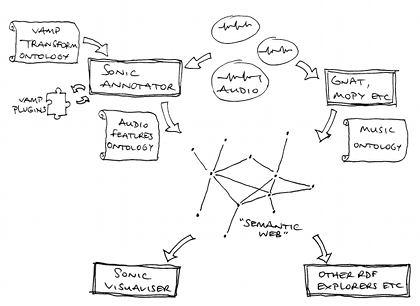
\includegraphics[width=0.7\textwidth]{img/semantic-web-and-friends-webscale.png} 
\caption{Workflow diagram of Sonic Annotator and Visualizer} \label{fig:sonic}
\end{figure}

\begin{figure}
\centering
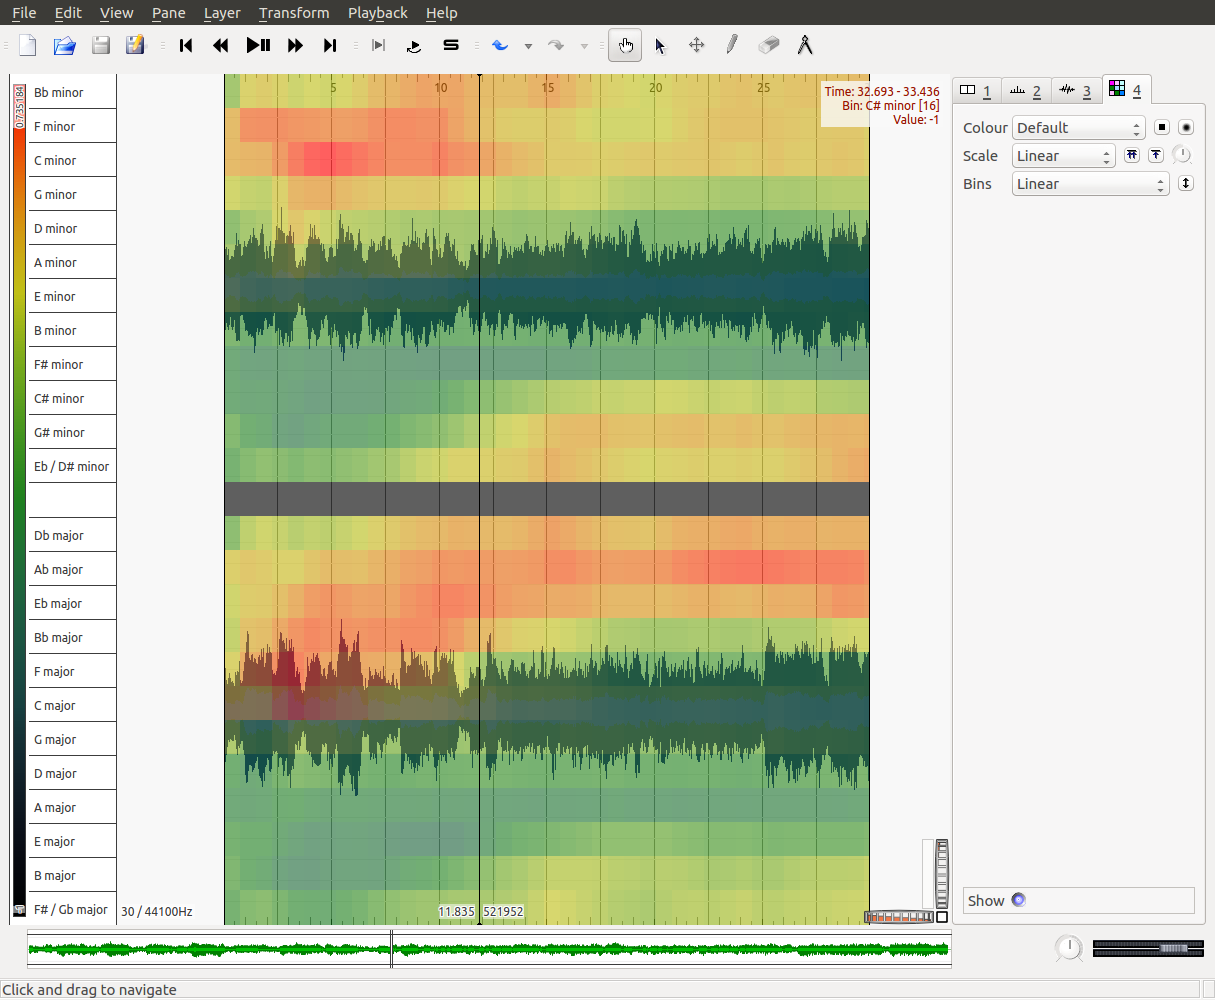
\includegraphics[width=0.7\textwidth]{img/sonic_visualizer.png} 
\caption{Bach Prelude 568 fragment with Key Strength Plot in Sonic Visualizer} \label{fig:sonic}
\end{figure}

\subsection{Python}

\subsection{Bash}

\subsection{MATLAB}

\subsection{Deep Learn Toolbox}



\section{Feature extraction}\label{sec:feature_extraction}


\subsection{Key Mode}\label{subsec:keymode}

The Vamp Plugin "Key Mode" calculates the major or minor mode of the estimated key in windows of 10 chroma frames. After calculate them, I use the count of the changes between minor and major as a feature.

\subsection{Segmentation}\label{subsec:segmentation}

This is also feature from a Vamp Plugin from Queen Mary which divides the channel into 10 structural segments based on Chroma and MFCC. Also, it labels similar segments, which gives us a structural analysis of the sample based on tonality. As key mode, I also use the count of the segments that appear at the segment.

\subsection{Tonality}\label{subsec:chord_windows}

The main work has been done in these following high level features based on the key of the sample and the detected chords. First of all, I obtain through the key strength Vamp plugin the value between -1 and 1 of every key (from C, C\#, and so on, to B minor and major) of every window of 1 chroma frame. Then, I select the most strong key of every window.

This set of windows, then, need to be transposed to convert this incontextual chords into a functional chords to get a functional harmonic analysis of the sample. To transpose, I created a script in Python that use the key of the sample, which I obtain using a weighted sum of the number of perfect cadences found at the key strength using 1 chroma, and the values of key strength plugin using 10 chroma. This key is used as a feature.

\subsection{Harmonic analysis}\label{subsec:uni_bi_tri}

From the previous feature we can obtain the number of functional units in the sample (tonic, dominant, subdominant, etc.), the number of most used cadences (perfect authentic cadence, plagal cadence, half-cadence, etc.) and even a set of most used progressions of three chords (like IV-V-I). As a parallelism of the POS tagging in text, is interesting to analyse the impact of this features because it's known that discriminate the composers \cite{desportes}.

\subsection{MFCC means}\label{subsec:mfcc_means}
At last, I included the means of the MFCC (Vamp Plugin) from the sample, using 20 coefficients and including C0, also to compare this low level feature with the previous ones.


\section{Classification}\label{sec:classification}

In the proposed systems, I used a Neural Network (NN) in one system and a Deep Belief Network (DBN) in another one to pre-train a Neural Network as a classifiers implemented by Rasmus Berg \cite{IMM2012-06284}. The features are normalized with z-score and after that, normalized between 0 and 1 before using the neural network. The networks are configured with 44 neurons at the hidden layer, 300 epochs, a batch size based on a divisor of the number of dataset samples, sigmoid activation function and softmax function at the output layer. I tested the system with a homemade database of FLAC files, extracted from my own CD's of the authors of the task.

\begin{figure}
\begin{center}
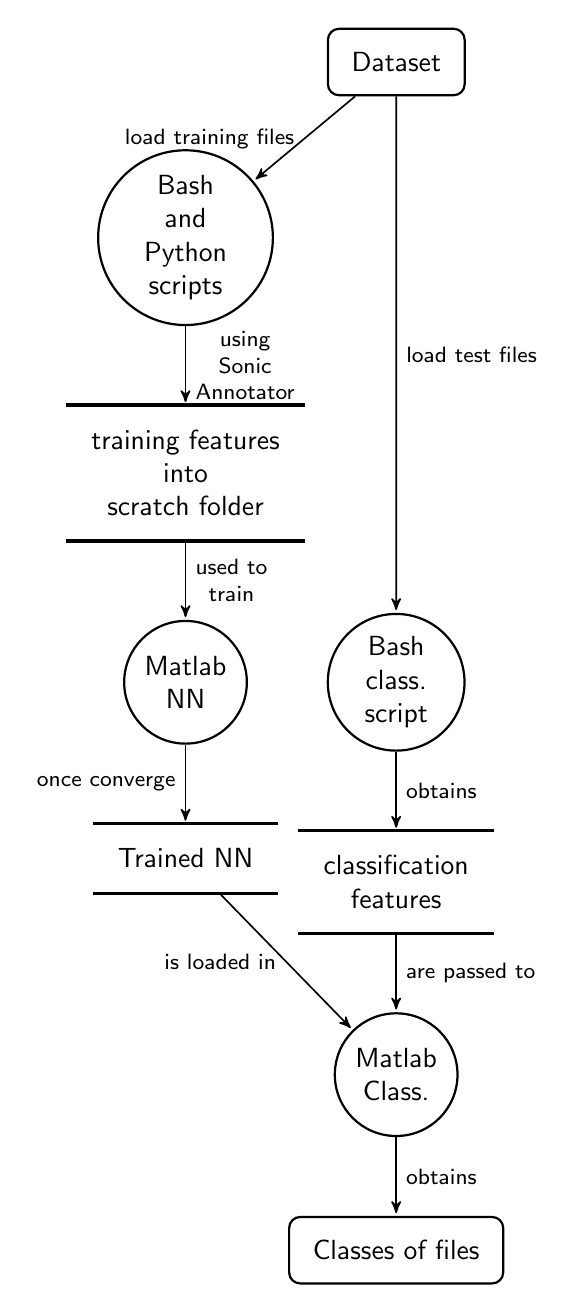
\begin{tikzpicture}[
  font=\sffamily,
  every matrix/.style={ampersand replacement=\&,column sep=2cm,row sep=2cm},
  source/.style={draw,thick,rounded corners,inner sep=.3cm},
  process/.style={draw,thick,circle},
  sink/.style={source},
  datastore/.style={draw,very thick,shape=datastore,inner sep=.3cm},
  dots/.style={gray,scale=2},
  to/.style={->,>=stealth',shorten >=1pt,semithick,font=\sffamily\footnotesize},
  every node/.style={align=center}]

  % Position the nodes using a matrix layout
    \node[source] (dataset) {Dataset};
      \node[process, below left = of dataset] (bps) {Bash\\and\\Python\\scripts};
      \node[datastore, below = of bps] (Tfeatures) {training features\\into\\scratch folder};
      \node[process, below = of Tfeatures] (NN) {Matlab\\NN};
      \node[datastore, below = of NN] (trained_nn) {Trained NN};
      \node[process, right = of NN] (bcs) {Bash\\class.\\script};
      \node[datastore, below = of bcs] (Cfeatures) {classification\\features};
      \node[process, below = of Cfeatures] (mat_class) {Matlab\\Class.};
      \node[sink, below = of mat_class] (classification) {Classes of files};


  % Draw the arrows between the nodes and label them.
  \draw[to] (dataset) -- node[midway,left] {load training files} (bps);
  \draw[to] (bps) -- node[midway,right] {using\\Sonic\\Annotator} (Tfeatures);
  \draw[to] (Tfeatures) -- node[midway,right] {used to\\train} (NN);
  \draw[to] (NN) -- node[midway,left] {once converge} (trained_nn);
  \draw[to] (dataset) -- node[midway,right] {load test files} (bcs);
  \draw[to] (trained_nn) -- node[midway,left] {is loaded in} (mat_class);
  \draw[to] (bcs) -- node[midway,right] {obtains} (Cfeatures);
  \draw[to] (Cfeatures) -- node[midway,right] {are passed to} (mat_class);
  \draw[to] (mat_class) -- node[midway,right] {obtains} (classification);
\end{tikzpicture}
\caption{Workflow of the proposed system}
\end{center}
\end{figure}

\newpage
\thispagestyle{empty}
\mbox{}


\chapter{Experiments}\label{experiments}
For the experiments, I used a database created by myself. The reason for this decision is that music database are not easy to distribute because of copyright issues.

The database I created is structured exactly the same way that the MIREX task specifies:

\begin{quote}
\begin{itemize}
\item 2772 30-second 22.05 kHz mono wav clips
\item 11 "classical" composers (252 clips per composer), including:
	\begin{itemize}
	\item Bach
	\item Beethoven
	\item Brahms
	\item Chopin
	\item Dvorak
	\item Handel
	\item Haydn
	\item Mendelssohn
	\item Mozart
	\item Schubert
	\item Vivaldi 
	\end{itemize}
\end{itemize}
\end{quote}

The disks I used are (respectively to each composer):
\begin{itemize}
\item 2772 30-second 22.05 kHz mono wav clips
\item 11 "classical" composers (252 clips per composer), including:
	\begin{itemize}
	\item Bach - The Baroque Music Library (\url{http://www.baroquemusiclibrary.com/})
	\item The Very Best of Beethoven
	\item The Best of Brahms
	\item Chopin - Complete Edition (Deutsche Grammophon)
	\item The Very Best of Dvorak
	\item Handel - The Baroque Music Library (\url{http://www.baroquemusiclibrary.com/})
	\item Haydn - The Baroque Music Library (\url{http://www.baroquemusiclibrary.com/})
	\item Mendelssohn - The complete symphonies
	\item Mozart - Complete Works 
	\item Franz Schubert - Masterworks
	\item The Very Best of Vivaldi 
	\end{itemize}
\end{itemize}


After downloading (most of them in MP3) and dumping the audios into WAV files using Asunder app, I created a "quick" bash command to convert all .mp3 files into WAV:
\lstset{language=Bash,
           basicstyle=\ttfamily\scriptsize,
           keywordstyle=\ttfamily,
           stringstyle=\ttfamily,
           commentstyle=\ttfamily,
          breaklines=true
          }
\begin{lstlisting}
find * -type f -name "*.mp3"  -exec avconv -i '{}' '{}.wav'
\end{lstlisting}

And also another one to cut all files into 30 seconds fragments and classified in folders by composer:
\lstset{language=Bash,
           basicstyle=\ttfamily\scriptsize,
           keywordstyle=\ttfamily,
           stringstyle=\ttfamily,
           commentstyle=\ttfamily,
          breaklines=true
          }
\begin{lstlisting}
for FOLDER in `ls`; do cd $FOLDER; rename 's/^(.{30}).*(\..*)$/$1$2/' * && find | rename 's/[\ \-(),;]//g' && COUNTER=1; for FILE in `ls`; do LENGTH=`nohup sox $FILE -n stat | grep "Length (seconds):" | sed 's/\ //g' | cut -f 2 -d ':' | cut -f 1 -d '.'`; LENGTH=$(( LENGTH - 30 )); LENGTH=${LENGTH/#-/}; for i in 1 2 3 4 5 6 7 8 9 10 11 12 13 14 15 16 17 18 19 20; do STARTVALUE=`echo $RANDOM % $LENGTH + 1 | bc`; COMMAND="sox "$FILE" "${COUNTER}_$FILE" trim $STARTVALUE 30"; COUNTER=$((COUNTER+1)); echo $COMMAND; eval $COMMAND; done ; rm $FILE; done; cd ..; done
\end{lstlisting}

Also, to test the workflow of the MIREX task, I created the list of files for feature extraction, training and classification with another simple Bash script:

\lstset{language=Bash,
           basicstyle=\ttfamily\scriptsize,
           keywordstyle=\ttfamily,
           stringstyle=\ttfamily,
           commentstyle=\ttfamily,
          breaklines=true
          }
\begin{lstlisting}
find /home/leopoldo/tfm/audio/ -type f > featureExtractionFiles.txt
cat featureExtractionFiles.txt | cut -f 6 -d '/' > tmp
paste featureExtractionFiles.txt tmp > trainingFiles.txt
find /home/leopoldo/tfm/audio-testing/ -type f > classifyFiles.txt
cat classifyFiles.txt | cut -f 6 -d '/' > tmp
paste classifyFiles.txt tmp > expectedResult.txt
rm tmp
\end{lstlisting}


This created an amount of 2420 files (6.4GB), but due to the length gap between authors, I decided to delete some audio fragment from some composers and created a final corpus of 1100 files (2.100 files per author).

So, I experimented with my dataset focusing on the harmonic analysis because that features were implemented by myself. I experimented with different Neural Network configurations, with DBN and NN, and using different groups of features to compare the impact of each of them using a three-fold cross validation process.


\begin{figure}
\centering

   \begin{tabular}{ | l | l || l | l |}
   \hline
   Features & \# of features & DBN & NN \\ \hline
   Means MFCC & 20 & 33.5 & \bf{37.1} \\ \hline
   Means MFCC + Segmentation + Major/Minor & 32 & \bf{27.8} & 25.9 \\ \hline
   Harmonic Analysis + Means MFCC & 68 & 28.0 & \bf{35.3}\\ \hline
   All & 80 & 18.1 & \bf{29.7} \\ \hline
   \end{tabular}

\caption{Average three-fold cross-validation accuracies, in percent. Moldface: best performance for a given setting (row).} \label{fig:results}
\end{figure}


The results are approximate because the MIREX Train/Test tasks are not finished at the submission deadline of this paper.

\newpage
\thispagestyle{empty}
\mbox{}


\chapter{Conclusions}\label{conclusions}


\section{Future work lines}





\nocite{*}
\cleardoublepage
\addcontentsline{toc}{chapter}{Bibliography}
\bibliographystyle{ieeetr}
\bibliography{bibliography}




\newpage
\thispagestyle{empty}
\mbox{}


\appendix
\chapter{Donwload links}\label{links}
\begin{itemize}

\item Download this document: \url{https://github.com/Lesbinary/TFM/raw/master/doc/report.pdf}

\item Source code download (documentation and implementation): \url{https://github.com/Lesbinary/tfm/archive/master.zip}

\item Github Repository: \url{https://github.com/Lesbinary/tfm}

\item GPLv3 License: \url{https://github.com/Lesbinary/tfm/blob/master/LICENSE}

\end{itemize}


\chapter{Environment configuration}\label{configuration}

This project has been developed under clean install of Ubuntu 15.04 but it also works on Ubuntu 14.04 LTS. The only needed software that is not installed by default is MATLAB and I used version 2014a.

First of all, you need to download my repository (see appendix \ref{links}) into the folder you want. After that, you need to copy the "vamp" folder of the root of the repository into your home folder (\$HOME/vamp) or into /usr/local/lib/vamp because Sonic Annotator searches for plugins in that paths.

Then you are ready to use the script based on the standard of MIREX submissions (\url{http://www.music-ir.org/mirex/wiki/2015:Audio_Classification_%28Train/Test%29_Tasks#Example_submission_calling_formats}), for example:
   \lstset{language=Bash,
           basicstyle=\ttfamily\scriptsize,
           keywordstyle=\ttfamily,
           stringstyle=\ttfamily,
           commentstyle=\ttfamily,
          breaklines=true
          }
\begin{lstlisting}
	tfmFeatureExtractor.sh -numThreads 8 ~/tfm/scratch/ ~/tfm/trunk/featureExtractionFiles.txt
	tfmTrainer.sh -numThreads 8 ~/tfm/scratch/ ~/tfm/trunk/trainingFiles.txt
	tfmClassifier.sh -numThreads 8 ~/tfm/scratch/ ~/tfm/trunk/classifyFiles.txt  ~/tfm/trunk/finalResult
\end{lstlisting}
	
And that's it. Also keep in mind that you will need a system with at least 80MB. It's recommended 100-150MB for using a corpus like the one in MIREX. Also keep in mind that there is an option of multithreading which can improve the speed of the run. The default threads value is 4 and can be set with the parameter "-numThreads" (see previous example).

\end{document}
\grid
